\section{Basis-Konvertierung ganzer Zahlen}

Die Notation $[9]_{10}$ bedeutet, dass man die Zahl 9 im Zehner-System betrachtet. Es gilt also $[9]_{10} = [1001]_2$ und $[10]_{10}=[1010]_2$. 

Um eine Zahl von einer gegebenen Basis in eine Zielbasis $b$ zu konvertieren, so teilt man immer wieder durch $b$ und notiert den Rest als nächste Ziffer von hinten nach vorne. Am Beispiel von $[57]_{10}$ ins Zweier-System sieht das so aus:
\begin{align}
	\frac{57}{2} &= 28\text{ Rest } 1 \Rightarrow\text{ letzte Ziffer der Binärdarstellung} \notag \\
	\frac{28}{2} &= 14\text{ Rest } 0 \Rightarrow\text{ vorletzte Ziffer der Binärdarstellung} \notag \\
	\frac{14}{2} &= 7\text{ Rest } 0 \notag \\
	\frac{7}{2} &= 3\text{ Rest } 1 \notag \\
	\frac{3}{2} &= 1\text{ Rest } 1 \notag \\
	\frac{1}{2} &= 0\text{ Rest } 1 \notag
\end{align}
Also gilt: $[57]_{10}=[111001]_2$.

Die umgekehrte Richtung verläuft ähnlich:
\begin{center}
	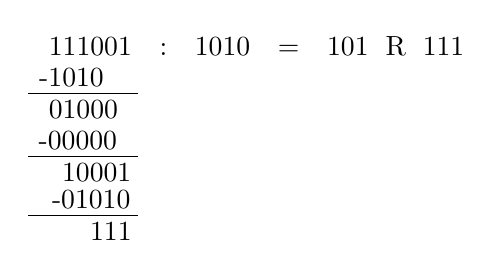
\begin{tikzpicture}
		\node at (0,0) (a) {111001\quad :\quad 1010\quad =\quad 101\; R\; 111};
		\node at (-2.35,-0.4) (b) {-1010};
		\draw (-2.9,-0.6) -- (-1.5,-0.6);
		\node at (-2.2, -0.8) (c) {01000};
		\node at (-2.27, -1.2) (d) {-00000};
		\draw (-2.9,-1.4) -- (-1.5,-1.4);
		\node at (-2.03,-1.6) (e) {10001};
		\node at (-2.1,-1.95) (f) {-01010};
		\draw (-2.9,-2.15) -- (-1.5,-2.15);
		\node at (-1.85,-2.35) (g) {111};
	\end{tikzpicture}
\end{center}
Also $[111001]_2$ durch $[10]_{10}=[1010]_2$ gleich $[101\text{ Rest }111]_2=[5\text{ Rest }7]_{10}\Rightarrow [57]_{10}$.

Von Basis 2 in Basis 4, 8 oder 16 ist dann ganz einfach: $[111100101]_2$
\begin{itemize}
	\item Zweiergruppen von hinten nach vorne zusammenzählen: $[13211]_4$
	\item Dreiergruppen von hinten nach vorne zusammenzählen: $[745]_8$
	\item Vierergruppen von hinten nach vorne zusammenzählen: $[1E5]_{16}$
\end{itemize}